
%What is an auto encoder
\subsection{Autoencoder}
An autoencoder \cite{hinton2006reducing} is a type of artificial neural network designed to learn efficient representations of data, typically for the purpose of dimensionality reduction or feature learning through unsupervised learning. An autoencoder consists of two main components: an encoder and a decoder.\\

The encoder part of the network compresses the input 
$\mathbf{x} \in \R^n$ into a latent-space representation $\mathbf{z} \in \R^m$. Where $m < n$.

The encoder is defined by a function $\phi$:
$$
\mathbf{z}=\phi(\mathbf{x})
$$

The output of the encoder, $\mathbf z$, is known as the latent space representation or the code. This compressed representation captures the most important features of the input data, facilitating tasks such as denoising, anomaly detection, and data compression.

The decoder reconstructs the input data from the latent representation. Similar to the encoder, the decoder consists of one or more layers and is typically a mirror image of the encoder architecture. It is defined by another function $\psi$:
$$
\hat{\mathbf{x}}=\psi(\mathbf{z})
$$

The objective of an autoencoder is to minimize the reconstruction error, which measures the difference between the input $\mathbf{x}$ and the reconstructed output $\hat{\mathbf{x}}$. This is often done using a loss function $L$, such as the mean squared error:
$$
L(\mathbf{x}, \hat{\mathbf{x}})=\|\mathbf{x}-\hat{\mathbf{x}}\|^2
$$
The overall optimization problem is to find the weights and biases of both the encoder and decoder network that minimize this loss

%Hva er Sindy
\subsection{SINDy}

\begin{figure}[H]
    \centering
    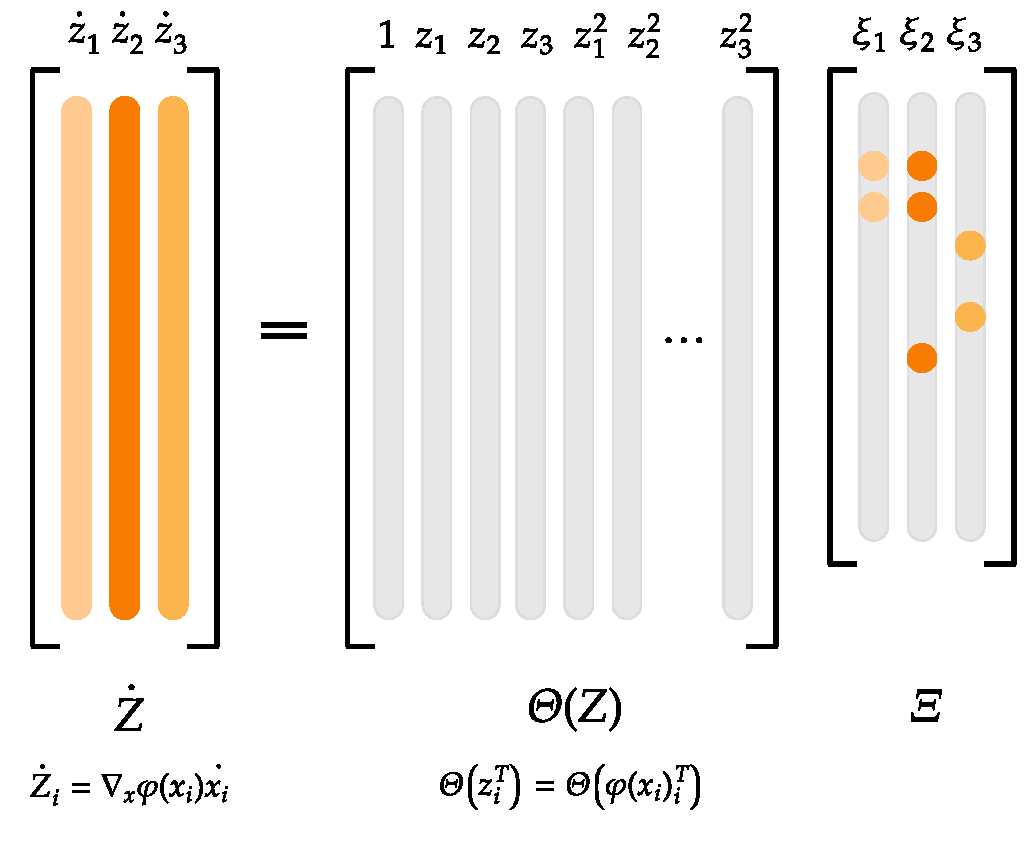
\includegraphics[width=0.48\textwidth]{project_2/images/SINDy_diagram.pdf}
    \caption{}
    \label{fig:SINDy_diagram}
\end{figure}

The SINDy (Sparse Identification of Nonlinear Dynamics) algorithm is a procedure first described in the paper \cite{Brunton_2016} for taking time-series data and extracting interpretable and generalizable dynamical system models that describe the data. If we use the SINDy algorithm on a dynamical system described by a differential equation:
$$
\frac{d \mathbf{x}}{d t}=\mathbf{f}(\mathbf{x})
$$
where $\mathbf{x} \in \mathbb{R}^n$ is the state vector, and $\mathbf{f}(\mathbf{x})$ represents the unknown nonlinear functions governing the system dynamics. Then the goal of SINDy is to identify $\mathbf{f}(\mathbf{x})$ from measurements of $\mathbf{x}$.
So if we have time-series data $\left\{\mathbf{x}\left(t_1\right), \mathbf{x}\left(t_2\right), \ldots, \mathbf{x}\left(t_m\right)\right\}$ and corresponding derivatives $\left\{\dot{\mathbf{x}}\left(t_1\right), \dot{\mathbf{x}}\left(t_2\right), \ldots, \dot{\mathbf{x}}\left(t_m\right)\right\}$ We can construct a library $\Theta(\mathbf{x})$ containing $p$ candidate functions that might describe the dynamics:
$$
\Theta(\mathbf{x})=\left[\begin{array}{llll}
\theta_1(\mathbf{x}) & \theta_2(\mathbf{x}) & \cdots & \theta_p(\mathbf{x})
\end{array}\right]
$$

Typical choices for $\Theta(\mathbf{x})$ include polynomials, trigonometric functions, and other nonlinear functions of the state variables. 

Furthermore we can express the time derivatives $\dot{\mathbf{x}}$ as a linear combination of the candidate functions:
$$
\dot{\mathbf{x}}=\Theta(\mathbf{x}) \boldsymbol{\Xi}
$$
where $\boldsymbol{\Xi} \in \mathbb{R}^{p \times n}$ is a sparse matrix of coefficients to be determined. The final goal of the SINDy algorithm is solving the sparse regression problem to find $\boldsymbol{\Xi}$ :
$$
\boldsymbol{\Xi}=\arg \min _{\boldsymbol{\Xi}}\|\dot{\mathbf{x}}-\Theta(\mathbf{x}) \boldsymbol{\Xi}\|_2+\lambda\|\boldsymbol{\Xi}\|_1
$$
where $\|\cdot\|_2$ is the $\mathrm{L} 2$ norm, $\|\cdot\|_1$ is the $\mathrm{L} 1$ norm promoting sparsity, and $\lambda$ is a regularization parameter. Once $\boldsymbol{\Xi}$ is determined, the non-zero entries in each column of $\boldsymbol{\Xi}$ correspond to the active terms in the governing equations for each state variable:
$$
\frac{d x_i}{d t}=\sum_{j=1}^p \xi_{ij} \theta_j(\mathbf{x})
$$
Where $\xi_{ij}$ denotes the indices of $\Xi$.

The reason we care about sparsity in the models is that it makes them more interpretable, and if they are every to be used for ciritical evaluations they need to be interpretable to be trusted.

\subsection{Symbolic regression}
SINDy is one of many methods within the broader category of symbolic regression. What differentiates SINDy from other methods is that it requires a predefined library of candidate terms where each suspected term is computationally costly to include. This can be a big assumption to make depending on the system of study. Other symbolic regression methods such as PySR \cite{cranmer2020discovering} are less limited in their space of potential solutions. PySR instead uses a library of operators which it applies through a genetic algorithm to its population of solutions. This lets PySR explore a broader space of potential models than SINDy, but SINDy might more easily find a sparse solution, since it has to rely on its library.

%Hva er autoencoder SINDY
\subsection{Autoencoder SINDy}

\begin{figure}[H]
    \centering
    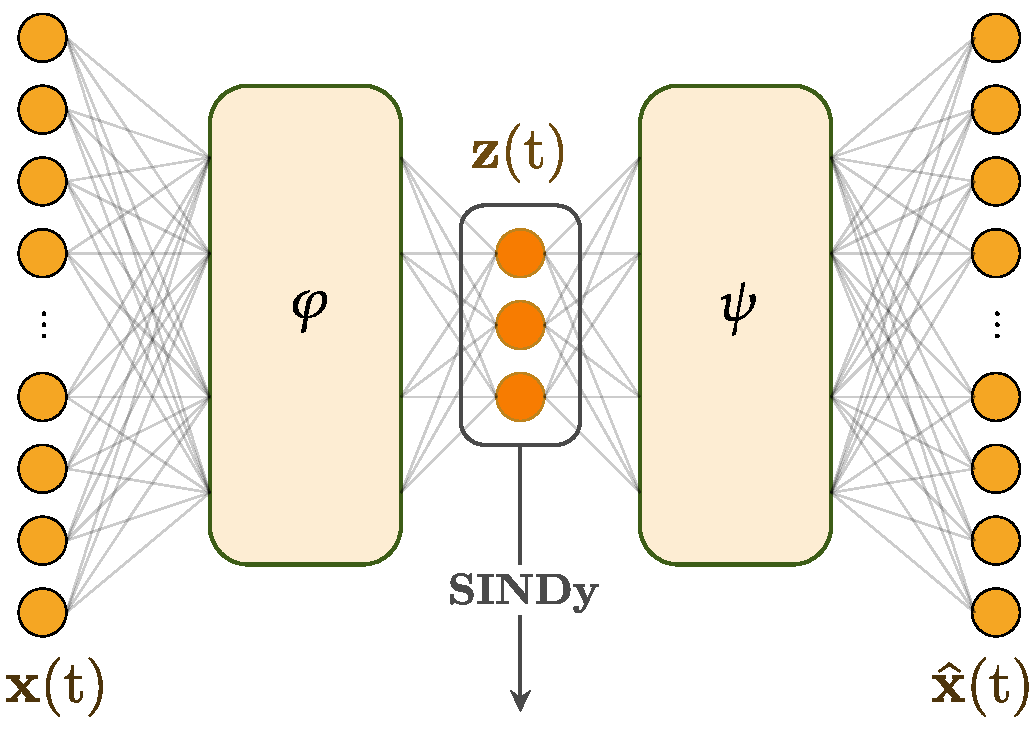
\includegraphics[width=0.48\textwidth]{project_2/images/autoencoder_diagram.pdf}
    \caption{}
    \label{fig:autoencoder_diagram}
\end{figure}

A drawback of using plain SINDy is that the data might be unnecessarily complex when represented in its original coordinates. A naive approach to solve this would be to apply an autoencoder to the data in isolation and then use SINDy on the possibly simpler latent space, i.e. solving for
\begin{equation}
    \dot{\mathbf{z}}=\Theta(\mathbf{z}) \boldsymbol{\Xi}.
\end{equation}
However, this does not ensure that the autoencoder coordinates learned will have associated sparse dynamical models. A further development to this issue is proposed by Champion et. al \cite{Champion_2019}. 

Champion's 2019 paper presents a method for the simultaneous discovery of sparse dynamical models and the coordinates that enable these simple representations. The paper details how to integrate a SINDy model with an autoencoder network to perform joint optimization. To ensure that the learned intrinsic coordinates have associated parsimonious dynamical models, the method incorporates the SINDy model into the autoencoder's training process. This is done by including terms in the loss function that enforce the accurate prediction of the dynamics in both the latent space and the original space. 

The library $\mathbf\Theta(\mathbf z)$ must still be decided beforehand, but the coefficients of $\mathbf\Xi$ are learned together with the autencoder parameters. Assuming that the time derivatives $\dot{\mathbf{x}}(t)$ of the original states are available or can be computed, the time derivatives of the encoder variables are given by:
\begin{equation}
    \dot{\mathbf{z}}(t)=\nabla_{\mathbf{x}} \phi(\mathbf{x}(t)) \dot{\mathbf{x}}(t)
\end{equation}

The SINDy loss term in the latent space is:
$$
\mathcal{L}_{d \mathbf{z} / d t}=\left\|\nabla_{\mathbf{x}} \phi(\mathbf{x}) \dot{\mathbf{x}}-\boldsymbol{\Theta}(\phi(\mathbf{x})) \boldsymbol{\Xi}\right\|^2
$$

Additionally, the loss term ensuring that SINDy predictions can reconstruct the time derivatives of the original data is:
$$
\mathcal{L}_{d \mathbf{x} / d t}=\left\|\dot{\mathbf{x}}-\left(\nabla_{\mathbf{z}} \psi(\phi(\mathbf{x}))\right) \boldsymbol{\Theta}(\phi(\mathbf{x})) \boldsymbol{\Xi}\right\|^2
$$
The overall loss function combines the reconstruction error, the SINDy model errors in both the latent space and the original space, and an L1 regularization term to promote sparsity of the coefficients:
\begin{equation}
    \mathcal{L}=\mathcal{L}_{\text {recon }}+\lambda_1 \mathcal{L}_{d \mathbf{x} / d t}+\lambda_2 \mathcal{L}_{d \mathbf{z} / d t}+\lambda_3\|\mathbf{\Xi}\|_1
\end{equation}
where $\lambda_1, \lambda_2$, and $\lambda_3$ are hyperparameters that determine the relative weighting of each term. In summary Champion achieves the joint discovery by optimizing the following loss:

% Dette hadde sett mye bedre ut på én linje
% Men vi har to kolonner fordi vi leker fysikere
\begin{align}
    \underbrace{\|\mathbf{x}-\psi(\mathbf{z})\|_2^2}_{\text {reconstruction loss }}
    +\underbrace{\lambda_1\left\|\dot{\mathbf{x}}-\left(\nabla_{\mathbf{z}} \psi(\mathbf{z})\right)\left(\boldsymbol{\Theta}\left(\mathbf{z}^T\right) \boldsymbol{\Xi}\right)\right\|_2^2}_{\text {SINDy loss in } \dot{\mathbf{x}}} \notag 
    \\
    +\underbrace{\lambda_2\left\|\left(\nabla_{\mathbf{x}} \mathbf{z}\right) \dot{\mathbf{x}}-\boldsymbol{\Theta}\left(\mathbf{z}^T\right) \boldsymbol{\Xi}\right\|_2^2}_{\text {SINDy loss in } \dot{\mathbf{z}}}+\underbrace{\lambda_3\|\boldsymbol{\Xi}\|_1}_{\begin{array}{c}\text { SINDy } \\ \text { regularization }\end{array}}
\end{align}
To ensure a parsimonious model, sequential thresholding is applied during training, setting coefficients below a certain threshold to zero at fixed intervals, effectively approximating L0 regularization.

The technique described by Champion reduces the complexity of the problem which potentially lets the joint autoencoder SINDy algorithm uncover the underlying structure of the problem more easily than the plain SINDy algorithm.

\subsection{Backpropagation}
Backpropagation is a supervised learning algorithm used for training artificial neural networks, particularly in the context of deep learning, such as for autoencoders. Backpropagation involves a forward pass to compute the network output and loss, followed by a backward pass to compute gradients. These gradients are then used to update the network's weights and biases, minimizing the loss function over successive iterations. \cite{backprop}. 

Consider a neural network with $L$ layers, where $l=1,2, \ldots, L$. Each layer $l$ has $n_l$ neurons. The input to the network is $\mathbf{x}$, and the output is $\hat{\mathbf{y}}$.

For each layer $l$ we can compute the weighted input $\mathbf{z}^{(l)}$ :
$$
\mathbf{z}^{(l)}=\mathbf{W}^{(l)} \mathbf{a}^{(l-1)}+\mathbf{b}^{(l)}
$$
where $\mathbf{W}^{(l)}$ is the weight matrix, $\mathbf{a}^{(l-1)}$ is the activation from the previous layer, and $\mathbf{b}^{(l)}$ is the bias vector. We can apply the activation function $g$ to obtain the next activation $\mathbf{a}^{(l)}$ :
$$
\mathbf{a}^{(l)}=g\left(\mathbf{z}^{(l)}\right)
$$
Then we can use this prediction to compute the loss function $\mathcal{L}(\hat{\mathbf{y}}, \mathbf{y})$ which quantifies the error between the predicted output $\hat{\mathbf{y}}$ and the true target output $\mathbf{y}$. Common loss functions include Mean Squared Error (MSE) and Cross-Entropy Loss. 

With the calculated loss we can use backpropogation to compute the gradient of the loss function with respect to each weight $\mathbf{W}^{(l)}$ and bias $\mathbf{b}^{(l)}$. 

The error $\delta^{(L)}$ at the output layer is given by:
$$
\delta^{(L)}=\nabla_{\mathbf{a}^{(L)}} \mathcal{L} \odot g^{\prime}\left(\mathbf{z}^{(L)}\right)
$$
where $\odot$ is the elementwise product, $\nabla_{\mathbf{a}^{(L)}} \mathcal{L}$ is the gradient of the loss function with respect to the activation $\mathbf{a}^{(L)}$, and $g^{\prime}$ is the derivative of the activation function. For each layer $l=L-1, L-2, \ldots, 1$, we propagate the error backwards:
$$
    \delta^{(l)}=\left(\mathbf{W}^{(l+1)}\right)^T \delta^{(l+1)} \odot g^{\prime}\left(\mathbf{z}^{(l)}\right)
$$
And compute the gradients of the loss function with respect to $\mathbf{W}^{(l)}$ and $\mathbf{b}^{(l)}$ :
$$
\begin{gathered}
\nabla_{\mathbf{W}^{(l)}} \mathcal{L}=\delta^{(l)}\left(\mathbf{a}^{(l-1)}\right)^T \\
\nabla_{\mathbf{b}^{(l)}} \mathcal{L}=\delta^{(l)}
\end{gathered}
$$
Then we update the weights and biases using the computed gradients:
$$
\begin{aligned}
\mathbf{W}^{(l)} & \leftarrow \mathbf{W}^{(l)}-\eta \nabla_{\mathbf{W}^{(l)}} \mathcal{L} \\
\mathbf{b}^{(l)} & \leftarrow \mathbf{b}^{(l)}-\eta \nabla_{\mathbf{b}^{(l)}} \mathcal{L}
\end{aligned}
$$
where $\eta$ is the learning rate.

\subsubsection{Lorenz}

\subsubsection{Legendre polynomials for Lorenz}
% hvordan input vektorer ser ut

 
